\section{PSoC Master implementering} \label{sec:PSoC_Master_impl}

Dette afsnit omhandler overvejelser og det udførte design for PSoC Master blokken i systemet.

\begin{figure}[h]
\centering
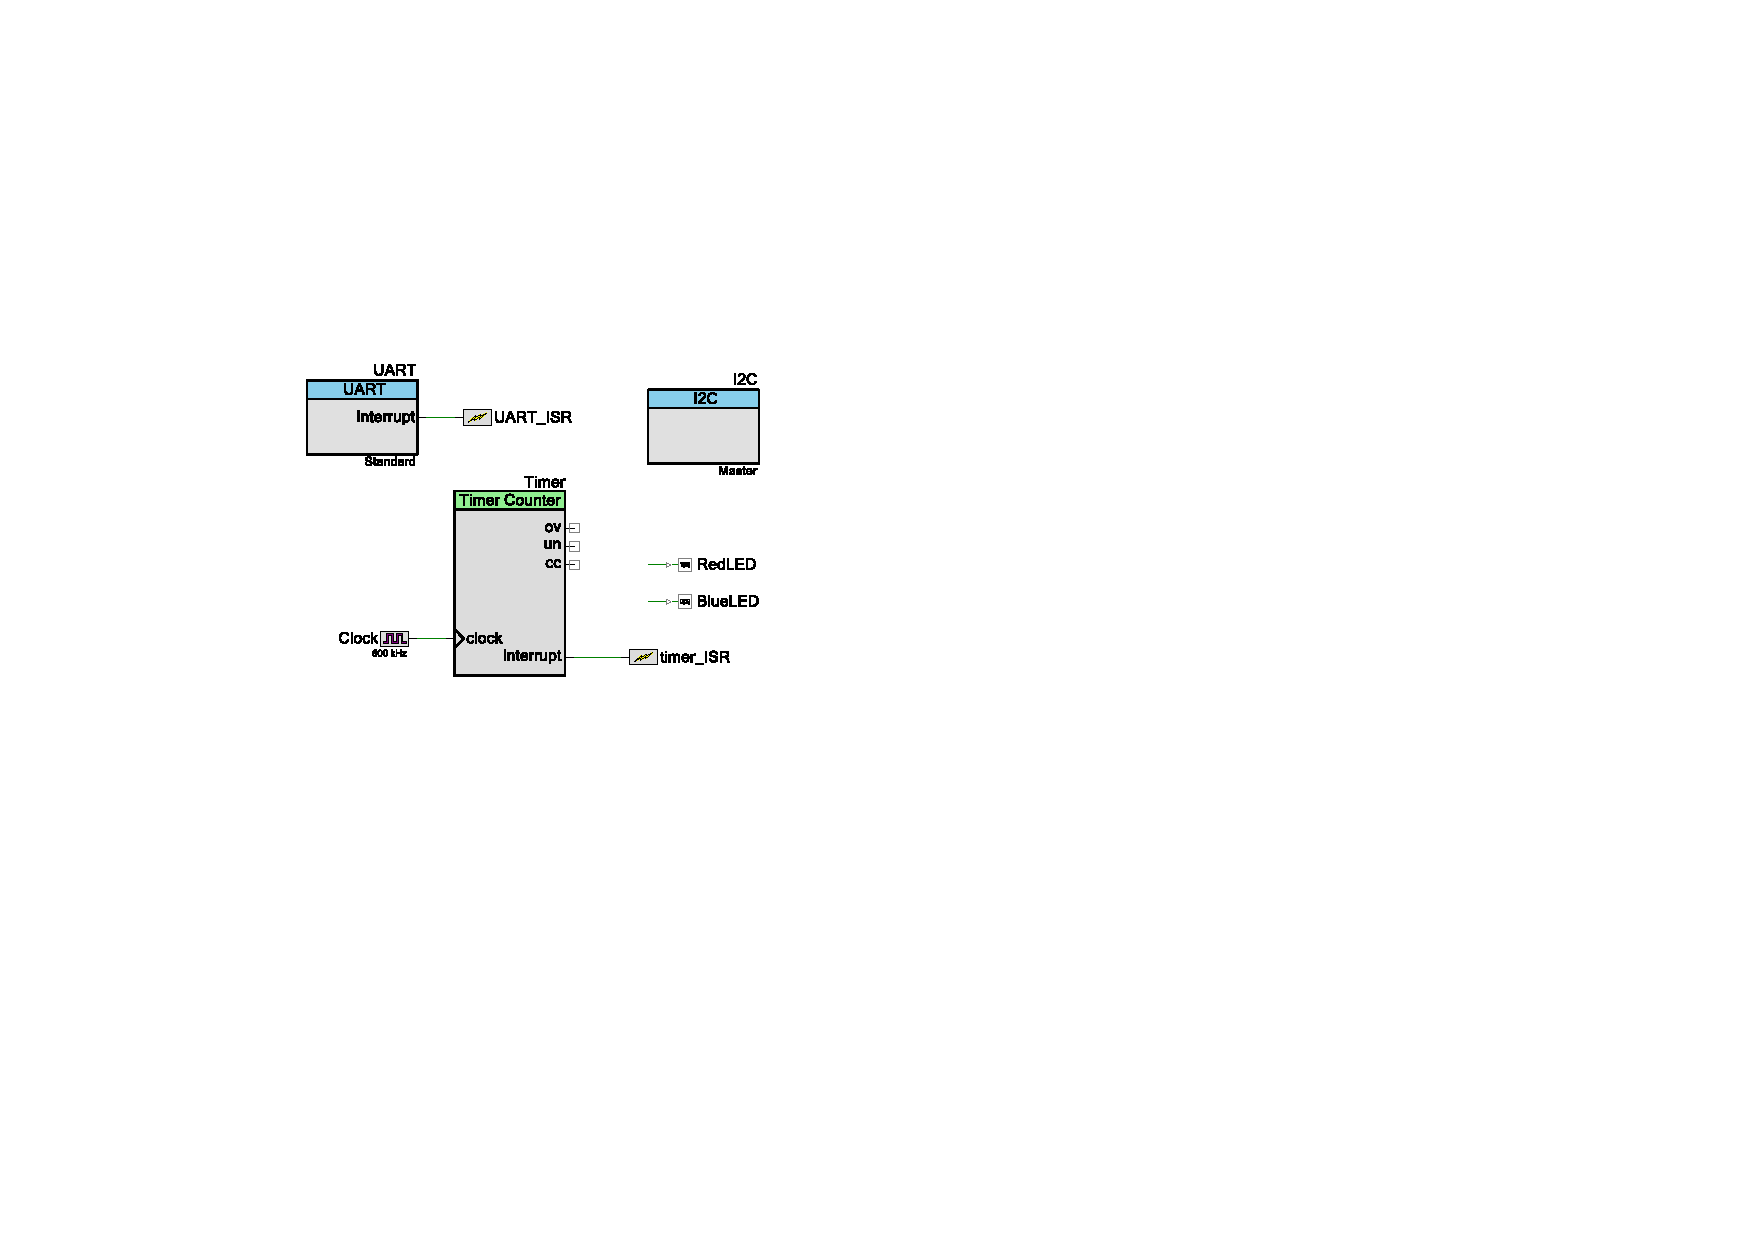
\includegraphics[width=\textwidth*3/5, trim=145 270 475 170, clip=true]{../fig/TopDesign_PSoC_Master}
\label{fig:psoc_master_topdesign}
\caption{TopDesign.cysch for PSoC\_Master}
\end{figure}

I Figur \ref{fig:psoc_master_topdesign} ses topdesignet for PSoC Master. Ud fra dette ses det at vi overordnet set har at gøre med en UART, som genererer interrupts, en Timer, som genererer interrupts, en I2C blok og to outputs til LED. 
Selve topdesignet er lavet ud fra de behov der er stillet i Design-fasen. Der blev under implementeringen af UART overvejet brug af en anden UART komponent, men problemet viste sig at ligge i et tidligere design-valg angående paritet.

\clearpage

\subsection{\IIC implementering}
%TODO Lasse skal kopiere tekst ind her.

\subsection{UART implementering}
UART klassen har til formål at modtage kommandoer fra DevKit8000, tolke disse og give passende svar. 

Generelt set er klassen implementering med udgangspunkt i vores UART protokol, men er udvidet således at der let kan implementeres flere trin i hhv. kontrol af vindue, motor og vanding. UART klassen gør brug af UART komponenten (SCB) vist i Figur \ref{fig:psoc_master_topdesign}.

\begin{lstlisting}[language=C,caption=Implementering af respondTemp(),label=lst:psoc_master_respondTemp]
int8 respondTemp(uint8 temp){
    if(temp){
        // If temp is between 1 and 200(both inclusive) "T" and temp is sent to DevKit8000
        UART_UartPutChar('T');
        UART_UartPutChar(temp);
        return 0;
    }
    else{
        // If temp isn't between 1 and 200(both inclusive) "XT" is sent to DevKit8000
        UART_UartPutChar('X');
        UART_UartPutChar('T');
        return -1;
    }
}
\end{lstlisting}

I Listing \ref{lst:psoc_master_respondTemp} vises et eksempel på en af funktionerne der håndterer svar via UART. De øvrige funktioner i klassen fungerer på samme måde. Funktionen modtager den værdi, der skal sendes tilbage til DevKit8000. Hvis parametren er 0 vil det sige at der er sket en fejl. Når funktionen kaldes kaldes den med returværdi fra DSP klassen, som beskrevet i afsnit \ref{sec:DSP_impl}.

\begin{lstlisting}[language=C, caption=Implementering af dkRequest(), label=lst:psoc_master_dkreq]
uint8 dkRequest(void){
    // Reads the UART buffer
    return UART_UartGetChar();
}
\end{lstlisting}

Vi har ydermere valgt at indkapsle læsningen fra UART ved hjælp af dkRequest() funktionen vist i Listing \ref{lst:psoc_master_dkreq}. 
Grunden til at vi har valgt at implementere denne er for at sikre os at hvis UART protokollen skulle ændre sig i fremtiden, kan disse ændringer tages højde for i denne funktion inden PSoC Master controllerklassen skal håndtere input fra UART.

\subsection{DSP implementering}\label{sec:DSP_impl}
DSP klassen agerer både digital signal processor og domæneklasse for vores måledata. 
Hver type af data er gemt i sit eget array, som vist i Listing \ref{lst:DSP_decl}. 
Hvert arrays har ligeledes en pointer til den næste plads i arrayet der skal overskrives.

\begin{lstlisting}[language=C, label=lst:DSP_decl, caption=Deklaration af arrays og pointers]
// Private data members
int32 tempArray[ARRAYSIZE];
int32* tempArrayPtr;
int32 humArray[ARRAYSIZE];
int32* humArrayPtr;
int16 soilHumArray[NBR_OF_SOILHUM_SENSORS][ARRAYSIZE];
int16* soilHumPtr[NBR_OF_SOILHUM_SENSORS];
int32 lightArray[ARRAYSIZE];
int32* lightArrayPtr;
uint8 temp, hum, soilHum[NBR_OF_SOILHUM_SENSORS], light;     // Used for storing the newest value
\end{lstlisting}



\subsection{Controller implementering}

PSoC\_Master controller-klassen er som udgangspunkt designet ud fra at blive styret af hvilke kommandoer der er modtaget på UART'en. På den måde agerer vores 'master' slave for DevKit8000. 
For at huske den nuværende status er der oprettet en \texttt{enum} med den nuværende status samt ekstra buffer til at holde styr på hvilken vandingsaktuator der modtages data omkring.

\begin{lstlisting}[language=C, label=lst:PSoC_m_dec, caption=Deklaration af buffers og flag.]
// Buffers / flags
typedef enum {IDLE, ADJW, ADJH, ADJV, ADJI} state;
volatile state theState = IDLE;
volatile int8 irrigationIndex = 0;
uint8 newByte = 0;
uint8 buff;
\end{lstlisting}

Ydermere er der lavet en form for debugging ved hjælp af de tre farvede LED'er på PSoC4 Pioneer Kit. Der tændes fx for den røde LED når et interrupt sker på timeren og for den blå når et interrupt sker på UARTen.

Når der sker et interrupt på UART'en, sættes flaget \texttt{newByte} til 1 og der fyldes data i bufferen. Dette ses i Listing \ref{lst:PSoC_m_uart_int}.

\begin{lstlisting}[language=C, label=lst:PSoC_m_uart_int, caption=ISR for UART.]
// UART ISR
CY_ISR(UART_ISR){
    newByte = 1;
    buff = dkRequest();
    UART_ClearRxInterruptSource(UART_GetRxInterruptSourceMasked());     // Clear interrupt flag
}
\end{lstlisting}

Årsagen til at vi har valgt at sætte et flag er at vi hurtigst muligt vil ud af interrupt service rutinen samt at det gav os problemer at have al funktionaliteten som kald fra UART ISR.

Der er herefter udarbejdet en ny privat funktion kaldet \texttt{uartIntHandler()},  %TODO Opdater navnet på inthandler
som sørger for at håndtere selve arbejdet mht. det input UART'en giver. 
Denne bliver kaldt med jævne mellemrum fra en \texttt{while(1)} løkke i main.c. 

\begin{lstlisting}[language=C, label=lst:PSoC_m_uartinth, caption=Interrupt handler for UART.]
void intHandler(){
    if (newByte){
        newByte = 0;
        BlueLED_Write(LED_ON);       // Turn on blue LED
        
        if(theState == IDLE){
            switch (buff){
                case 'T':{ //RequestTemp
                    respondTemp(getTemp_DSP());		
                    break;
                }
                case 'L':{ //RequestLight
                    respondLight(getLight_DSP());
                    break;
                }
                case 'A':{ //RequestAirhum
                    respondHum(getHum_DSP());
                    break;
                }        
                case 'H':{ //TurnHeatOn
                    // 0x7 is the maximum value.
                    respondHeat(adjustHeat(0x7), 'H');
                    break;
                }
                case 'K':{ //TurnHeatOff
                    // 0x0 is the minimum value.
                    respondHeat(adjustHeat(0x0), 'K');
                    break;
                }
                case 'W':{ //AdjustWindow
                    theState = ADJW;
                    break;
                }
                case 'V':{ //Ventilation
                    theState = ADJV;
                    break;
                }
                case 'F':{ //Watering
                    theState = ADJI;
                    break;
                }
                /*case 'S':{ //
                    respondSoilHum(); //TODO: Add stuff here
                    break;
                }*/
                default:{
                    // Do nothing - let the DevKit8000 timeout
                    break;
                }
            }
        }
        else if(theState == ADJW){
            if(buff-CONVERT_TO_ASCII == 1){
                respondWin(adjustWindow(0xFF));
            }
            else{
                respondWin(adjustWindow(0x00));
            }
            theState = IDLE;
        }
        else if(theState == ADJV){
            if(buff-CONVERT_TO_ASCII == 1){
                respondVent(adjustVentilation(0xFF));
            }
            else{
                respondVent(adjustVentilation(0x00));
            }
            theState = IDLE;
        }
        else if(theState == ADJI){
            if (!irrigationIndex){
                irrigationIndex = buff;
            }
            else{
                if (buff-CONVERT_TO_ASCII == 1){
                    respondIrri(adjustIrrigation(irrigationIndex-CONVERT_TO_ASCII-1, 0xFF));
                }
                else{
                    respondIrri(adjustIrrigation(irrigationIndex-CONVERT_TO_ASCII-1, 0x00));
                }
                irrigationIndex = 0;
                theState = IDLE;
            }
        }
        buff = 0;
        BlueLED_Write(LED_OFF);         // Turn off blue LED
    }
}
\end{lstlisting}

I Listing \ref{lst:PSoC_m_uartinth} ses implementeringen af selve interrupthandleren. Det ses hvordan der først tjekkes for om der er kommet ny data via \texttt{newByte} og der herefter kontrolleres hvilket stadie, systemet er i. Hvis det er i \texttt{IDLE} tjekkes der på hvad der står i bufferen og der udfærdes evt et svar eller ventes på næste databyte. Til at starte med tændes den blå LED og når kaldet er slut slukkes denne.

\clearpage